In order to accurately determine the position of the beam, the raster needs to be calibrated to the BPMs. Reading out the BPMs gives an accurate position, but it has a phase lag which causes the readout to be uncorrelated with the events it is recorded with. The raster current is read instantaneously, which means it is an accurate for the event it is recorded with. However, the raster current does not directly tell us the position of the beam. Using these two systems together, the BPMs give the spread of the beam and the raster current can then be mapped to this spread. When the transformation between the raster current and position is found, it is easy to have an accurate beam position for every event that is recorded.

\begin{figure}
	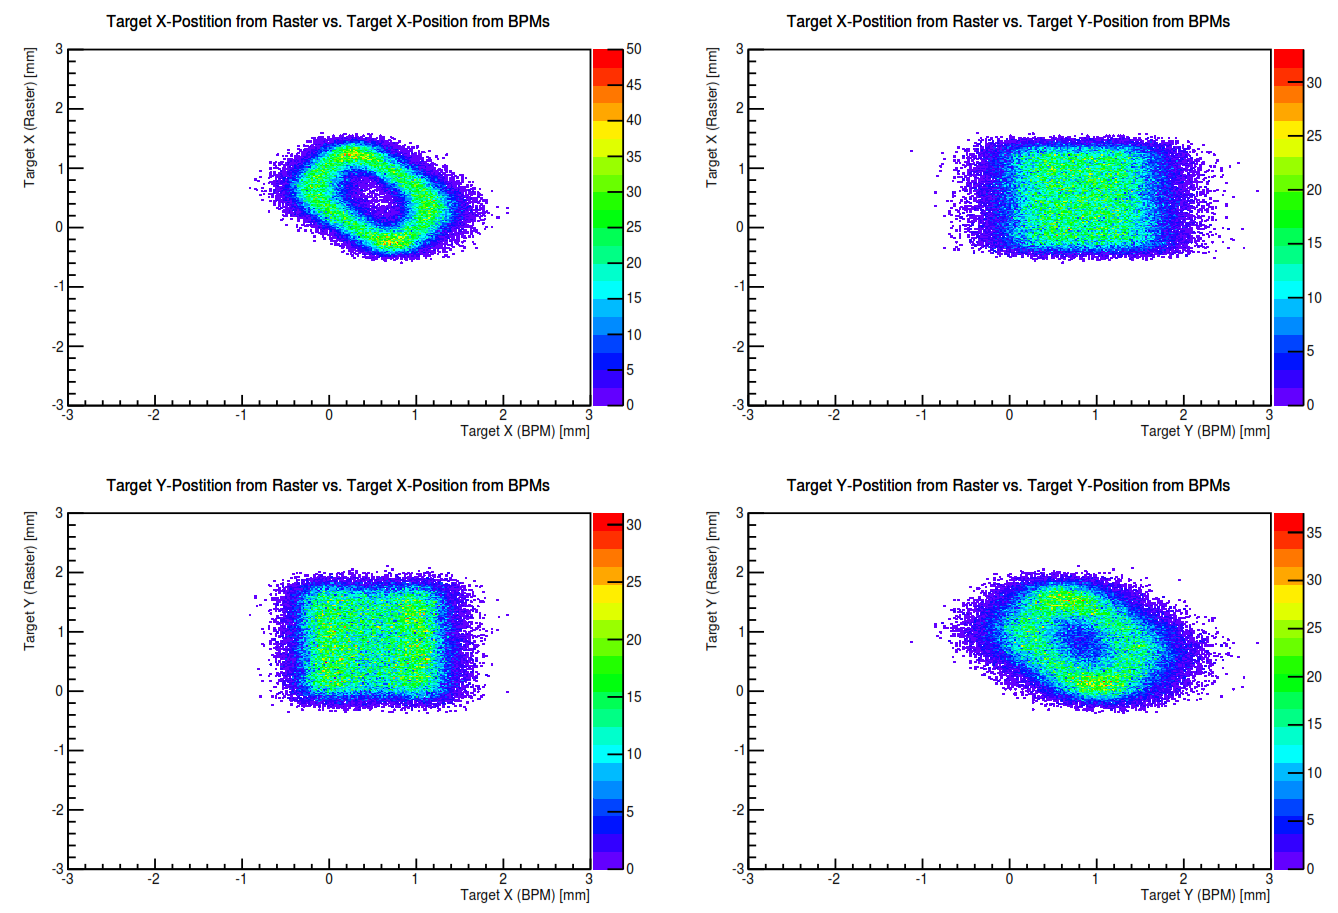
\includegraphics[width=\linewidth]{./chap3-analysis/fig/raster_bpm_sync.png}
	\caption{The BPM has a phase lag, causing the raster and BPMs to not be synced}
	\label{fig:raster}
\end{figure}